% Capítulo 11: a pilha ao longo de empilhar(1), empilhar(2), empilhar(3) e desempilhar.
\documentclass[border=4pt]{standalone}
\usepackage[utf8]{inputenc}
\usepackage[T1]{fontenc}
% Estilo comum das figuras de vetores (capítulo 8).
\usepackage{tikz}
\usetikzlibrary{arrows.meta, positioning, calc, decorations.pathreplacing}
\definecolor{navy}{RGB}{23,45,80}
\definecolor{laranja}{RGB}{250,110,29}
\definecolor{cinzalogo}{RGB}{107,114,126}
\definecolor{azul}{RGB}{205,222,247}
\tikzset{
  casa/.style={draw=navy, line width=0.9pt, minimum width=8mm, minimum height=7mm,
               inner sep=0pt, font=\sffamily\small},
  pronta/.style={casa, fill=azul},
  parte/.style={casa, fill=laranja!12},
  marcada/.style={casa, fill=laranja!45, draw=laranja},
  fora/.style={casa, draw=cinzalogo!60, dashed, fill=white, text=cinzalogo!60},
  indice/.style={font=\sffamily\scriptsize, text=cinzalogo},
  explica/.style={font=\sffamily\small, text=navy, anchor=east},
  legenda/.style={font=\sffamily\scriptsize, text=cinzalogo},
  rotulo/.style={font=\sffamily\small\bfseries, text=navy},
  seta/.style={-{Stealth[length=2.2mm]}, navy, line width=0.9pt},
  chave/.style={decorate, decoration={brace, amplitude=4pt, mirror}, navy, line width=0.8pt},
}
% \vetor{nome}{x}{y}{valor/estilo, valor/estilo, ...}: casas lado a lado, chamadas nome0, nome1...
\newcommand{\vetor}[4]{%
  \foreach \valor/\estilo [count=\i from 0] in {#4} {
    \node[\estilo] (#1\i) at ($(#2, #3) + (\i*0.8, 0)$) {\valor};
  }
}

\tikzset{
  casa/.append style={minimum width=10mm, minimum height=6mm},
  passo/.style={font=\ttfamily\scriptsize, text=navy, align=center},
}
% \estado{x}{valores de baixo para cima}{texto}
\newcommand{\estado}[3]{%
  \draw[navy, line width=0.9pt] (#1 - 0.65, 2.2) -- (#1 - 0.65, -0.35) -- (#1 + 0.65, -0.35) -- (#1 + 0.65, 2.2);
  \foreach \v [count=\k from 0] in {#2} {
    \node[pronta] at (#1, \k*0.6) {\v};
  }
  \node[passo] at (#1, -0.8) {#3};
}
\begin{document}
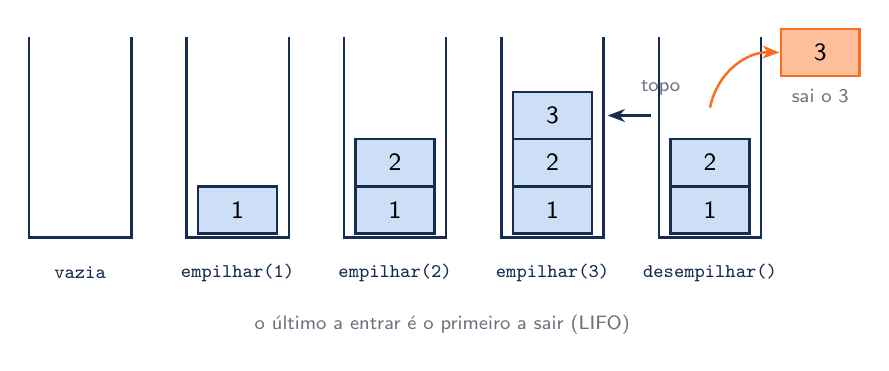
\begin{tikzpicture}
  \draw[navy, line width=0.9pt] (-0.65, 2.2) -- (-0.65, -0.35) -- (0.65, -0.35) -- (0.65, 2.2);
  \node[passo] at (0, -0.8) {vazia};
  \estado{2.0}{1}{empilhar(1)}
  \estado{4.0}{1, 2}{empilhar(2)}
  \estado{6.0}{1, 2, 3}{empilhar(3)}
  \estado{8.0}{1, 2}{desempilhar()}
  \node[marcada, minimum width=10mm, minimum height=6mm] (sai) at (9.4, 2.0) {3};
  \draw[seta, laranja] (8.0, 1.3) to[bend left=40] (sai.west);
  \node[legenda] at (9.4, 1.45) {sai o 3};
  \draw[seta] (7.25, 1.2) -- (6.7, 1.2);
  \node[legenda, anchor=west] at (7.0, 1.55) {topo};
  \node[legenda] at (4.6, -1.45) {o último a entrar é o primeiro a sair (LIFO)};
\end{tikzpicture}
\end{document}
